\chapter{Transmission Line Theory} \label{ch:TransmissionLineTheory}

Transmission line theory is needed for circuit analysis when the electrical size of the circuit is comparable to the wavelength which is is operating at. In lumped-circuit theory, the assumption is that the electrical size of the circuit is infinitely smaller than the wavelength. In RF and microwave circuits, the wavelength is on the order of millimetres, which is comparable to the electrical size of circuits that are fabricated at these frequencies (fractions or multiples of the wavelength), so transmission line analysis is required. A transmission line is a \coltextit{distributed parameter} network, hence, transmission line theory is sometimes call \coltextit{distributed circuit theory}. 

% *****************************************
% Lumped-Element Circuit Model 
% *****************************************
\section{Lumped-Element Circuit Model}
Any transmission line can be represented as a circuit with lumped elements as shown in Fig.\ \ref{fig:Ch1-TransmissionLineCircuit}. The parameters $R, L, G, C$ here are values per unit length (e.g. $R$ = series resistance per unit length in $\Omega/\text{m}$, $C$ = shunt capacitance per unit length in F/m, and so on). Hence, the equivalent resistance of the line for example is equal to $R\Delta z$ where $\Delta z$ is the length of the transmission line. 

\begin{figure}[!htp]
    \centering
    \begin{subfigure}{0.48\linewidth}
        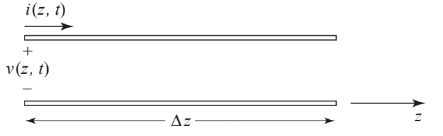
\includegraphics[width=\linewidth]{images/Transmission Line Theory/TransmissionLine-1.png}
        \caption{}
    \end{subfigure}
    \hfill
    \begin{subfigure}{0.48\linewidth}
        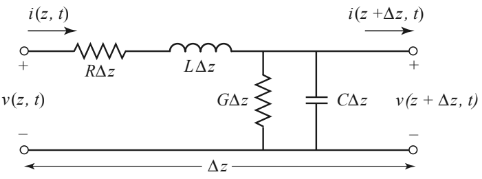
\includegraphics[width=\linewidth]{images/Transmission Line Theory/TransmissionLine-2.png}
        \caption{}
    \end{subfigure}
    \caption{(a) A tranmission line. (b) The equivalent lumped-circuit of the transmission line.}
    \label{fig:Ch1-TransmissionLineCircuit}
\end{figure}
The equations relating the current and voltage of the transmission lines are called the \coltextit{telegrapher equations} and are given in the time-domain as: 
\begin{empheq}[box=\eqnGreenBox]{align}
    \dfrac{\partial}{\partial t} v(z,t) &= -Ri(z,t) - L\dfrac{\partial}{\partial t} i(z,t) \\[2pt] 
    \dfrac{\partial}{\partial t} i(z,t) &= -Gv(z,t) - C\dfrac{\partial}{\partial t} v(z,t)
\end{empheq}
and in the phasor-domain:
\begin{empheq}[box=\eqnGreenBox]{align}
    \dfrac{d}{dz}\phasor{V}(z) &= -(R+j\omega L) \phasor{I}(z) \label{eq:TelegrapherEqn1} \\ 
    \dfrac{d}{dz}\phasor{I}(z) &= -(G+j\omega C) \phasor{V}(z) \label{eq:TelegrapherEqn2}
\end{empheq}

See Proof \ref{der:TelegrapherEquations} for how the telegrapher equations are obtained. 
\begin{proofBox}[Telegrapher Equations] \label{der:TelegrapherEquations}
    By Kirchoff's voltage and current laws, the following equations are obtained: 
    \begin{subequations}
    \begin{align}
        v(z,t) - R \Delta z\ i(z,t) - L \Delta z\ \dfrac{\partial}{\partial t}i(z,t) - v(z+\Delta z, t) &= 0 \\ 
        i(z,t) - G\Delta z \ v(z+\Delta z, t) - C\Delta z\ \dfrac{\partial}{\partial t}v(z+\Delta z, t) - i(z+\Delta z, t) &= 0 
    \end{align}
    \end{subequations}
    By rearranging the terms, the equations can be written as: 
    \begin{subequations}
    \begin{align}
        \dfrac{v(z+\Delta z, t) - v(z,t)}{\Delta z} &= -R i(z,t) - L\dfrac{\partial}{\partial t} i(z,t) \\ 
        \dfrac{i(z+\Delta z, t) - i(z,t)}{\Delta z} &= -Gv(z,t) - C\dfrac{\partial}{\partial t} v(z,t)
    \end{align}
    \end{subequations}
    Finally, by taking the limit as $\Delta z \to 0$ to both sides, we end up with the partial derivatives $\partial v(z,t)/\partial t$ and $\partial i(z,t)/\partial t$ on the left sides; the right sides are unaffected by the limit as there are no $\Delta z$ terms. And finally, we end up with the time-domain representation of the telegrapher equations:
    \begin{subequations}
    \begin{empheq}[box=\fbox]{align}
        \dfrac{\partial}{\partial t} v(z,t) &= -Ri(z,t) - L\dfrac{\partial}{\partial t} i(z,t) \\[2pt] 
        \dfrac{\partial}{\partial t} i(z,t) &= -Gv(z,t) - C\dfrac{\partial}{\partial t} v(z,t)
    \end{empheq}
    \end{subequations}
    Now let's perform the analysis in the phasor-domain. Using Kirchoff's voltage/current laws, we have: 
    \begin{subequations}
    \begin{align}
        \phasor{V}(z) - \phasor{I}(z)R\Delta z - \phasor{I}(z) j\omega L - \phasor{V}(z+\Delta z) &= 0 \\ 
        \phasor{I}(z) - (G\Delta z + j\omega C\Delta z)\phasor{V}(z) - \phasor{I}(z+\Delta z) &= 0
    \end{align}
    \end{subequations}
    Rearranging the equations, 
    \begin{subequations}
        \begin{align}
            \dfrac{\phasor{V}(z+\Delta z) - \phasor{V}(z)}{\Delta z} &= -(R+j\omega L) \phasor{I}(z) \\ 
            \dfrac{\phasor{I}(z+\Delta z) - I(z)}{\Delta z} &= -(G+j\omega C) \phasor{V}(z)
        \end{align}
    \end{subequations}
    And taking the limit as $\Delta z \to 0$, we have the telegrapher equations in the phasor-domain: 
    \begin{subequations}
    \begin{empheq}[box=\fbox]{align}
        \dfrac{d}{dz}\phasor{V}(z) &= -(R+j\omega L) \phasor{I}(z) \\ 
        \dfrac{d}{dz}\phasor{I}(z) &= -(G+j\omega C) \phasor{V}(z)
    \end{empheq}
    \end{subequations}
\end{proofBox}

% *****************************************
% Wave Propagation on a Transmission Line
% *****************************************
\section{Wave Propagation on a Transmission Line}
From solving Eqs.\ (\ref{eq:TelegrapherEqn1}) and (\ref{eq:TelegrapherEqn2}), the wave equations for $\phasor{V}(z)$ and $\phasor{I}(z)$ are obtained: 
\begin{empheq}[box=\eqnGreenBox]{align}
    \dfrac{d^2}{dz^2}\phasor{V}(z) - \gamma^2 \phasor{V}(z) &= 0 \label{eq:WaveEqn1} \\ 
    \dfrac{d^2}{dz^2} \phasor{I}(z) - \gamma^2 \phasor{I}(z) &= 0 \label{eq:WaveEqn2}
\end{empheq}
where $\gamma$ is the complex propagation constant
\begin{equation}
    \gamma = \alpha + j\beta = \sqrt{(R+j\omega L)(G+j\omega C)} \label{eq:PhaseContant}
\end{equation}
$\alpha$ is called the attenuation constant, and $\beta$ is the phase constant. The solution to Eqs. (\ref{eq:WaveEqn1}) and (\ref{eq:WaveEqn2}) is 
\begin{empheq}[box=\eqnGreenBox]{align}
    \phasor{V}(z) &= V_0^+ e^{-\gamma z} + V_{0}^- e^{\gamma z} \label{eq:VoltageEqn} \\ 
    \phasor{I}(z) &= I_0^+e^{-\gamma z} + I_0^- e^{\gamma z} \label{eq:CurrentEqn}
\end{empheq}
where the $e^{-\gamma z}$ term represents wave propagation in the $+z$ direction, and $e^{\gamma z}$ represents wave propagation in the $-z$ direction. The constants $V_0^+$ and $V_0^-$ (or $I_0^+$ and $I_0^-$) are unknown but can be determined if the source and load of the transmission line are known. Note that these constants are complex numbers. 
\begin{subequations}
\begin{align}
    V_0^+ = |V_0^+| e^{j\phi^+} \\ 
    V_0^- = |V_0^-| e^{j\phi^-}
\end{align}
\end{subequations}
%
\begin{note}[The Complex Propagation Constant] \phantom \newline
\begin{itemize}
    \item The propagation constant characterizes how the voltage/current changes along the transmission line.

    \item The attenuation constant tells us how lossy the line is; $\alpha=0$ means the line is lossless whereas $\alpha > 0$ means the line is lossy. The units are Nepres per metre, Np/m.

    \item The phase constant represents the rate at which the phase of the travelling wave along the line varies, and has units of rad/m. 
\end{itemize}
\end{note}
%
The characteristic impedance of the transmission line, $Z_0$, is defined as 
\begin{empheq}[box=\eqnGreenBox]{equation}
    Z_0 = \dfrac{V_0^+}{I_0^+} = \dfrac{-V_0^-}{I_0^-} = \dfrac{R+j\omega L}{\gamma} = \sqrt{\dfrac{R+j\omega L}{G + j\omega C}} \label{eq:CharacteristicImpedance}
\end{empheq}
The current along the transmission line can then be written as 
\begin{equation}
    \phasor{I}(z) = \dfrac{V_0^+}{Z_0} e^{-\gamma z} - \dfrac{V_0^-}{Z_0} e^{\gamma z}
\end{equation}
%
\begin{note}[The Characteristic Impedance $Z_0$] \phantom \newline
\begin{itemize}
    \item The characteristic impedance $Z_0$ is defined as the ratio of the incident voltage to current wave. 
    \item It is not to be confused with the electrical impedance. E.g., if $Z_0 = 50\ \Omega$, this does not mean that the transmission line is equivalent to a lumped $50\ \Omega$ resistor. 
    \item Eq.\ \ref{eq:CharacteristicImpedance} may be used to find the values of the equivlent lumped components of the line. 
\end{itemize}
\end{note}
%
The phase velocity of a wave along a transmission line is 
\begin{equation}
    v_p = \dfrac{\omega}{\beta} = \dfrac{1}{\sqrt{LC}}
\end{equation}
The corresponding wavelength of a wave travelling on the transmission line is then 
\begin{empheq}[box=\eqnGreenBox]{align}
    \lambda_g = \dfrac{v_p}{f} = \dfrac{2\pi}{\beta}
\end{empheq}
$\lambda_g$ is called the guided wavelength. 
%
\begin{note}[Phase Velocity $v_p$ and Guided Wavelength $\lambda_g$] \phantom \newline 
\begin{itemize}
    \item The phase velocity only represents the velocity of the wavefront; that is to say, the velocity of the peaks of a wave for a single frequency/wavelength. The phase velocity may be larger/smaller than the speed of light $c$ depending on the medium. In free-space, $v_p = c$. 
    
    \item The group velocity is the velocity of which the entire wave/particle is travelling at, and this velocity cannot be larger than $c$. The group wave is essentially the sum of all the waves of individual wavelengths/frequencies that are travelling together (recall by the Fourier series that a sinusoidal wave can be expressed as the sum of waves of varying frequencies). If we're looking at just a wave-packet that only consists of one wavelength/frequency, then its phase velocity is equal to the group velocity. 

    \item In electromagnetic texts, you'll see $\lambda$ used by the author to denote either $\lambda_0$ (free-space wavelength) or $\lambda_g$. It is up to you determine the author's notation as one author may use $\lambda$ to refer to the guided wavelength while another will use it to refer to the free-space wavelength. But as a rule of thumb, in the context of transmission lines, $\lambda$ is $\lambda_g$. Otherwise, $\lambda$ is $\lambda_0$. 

    \item Throughout this document, I will explicitly denote the wavelength by $\lambda_g$ or $\lambda_0$ for clarity.
\end{itemize}
\end{note}

% --- Lossless Transmission Lines
\subsection{Lossless Transmission Lines} \label{sec:LosslessLines}
In a lossless transmission line, $R = G = 0$, so Eq. (\ref{eq:PhaseContant}) becomes 
\begin{equation}
    \gamma = \alpha + j\beta = j\omega\sqrt{LC}
\end{equation}
 or
\begin{subequations}
\begin{align}
    \alpha &= 0 \\ 
    \beta &= \omega\sqrt{LC}
\end{align}
\end{subequations}
The wavelength is then 
\begin{equation}
    \lambda_g = \dfrac{2\pi}{\beta} 
\end{equation}
A useful equation for $\beta$ in a lossless line is 
\begin{equation}
    \beta = \omega\sqrt{\mu\varepsilon} = \omega\sqrt{LC}
\end{equation}
where $\mu$ and $\varepsilon$ is the magnetic permeability and electric permittivity, respectively. \par 

The characteristic impedance becomes 
\begin{equation}
    Z_0 = \sqrt{\dfrac{L}{C}} 
\end{equation}
The general solutions for voltage and current become 
\begin{subequations} 
\begin{align}
    \phasor{V}(z) &= V_0^+ e^{-j\beta z} + V_0^- e^{j\beta z} \\ 
    \phasor{I}(z) &= \dfrac{V_0^+}{Z_0} e^{-j\beta z} - \dfrac{V_0^-}{Z_0} e^{j\beta z}
\end{align}
\end{subequations}

% *****************************************
% The Terminated Lossless Transmission Line
% *****************************************
\section{Terminated Transmission Lines} \label{sec:TerminatedLines}
Consider Fig.\ \ref{fig:TL_Load}.

\begin{figure}[!htp]
    \centering
    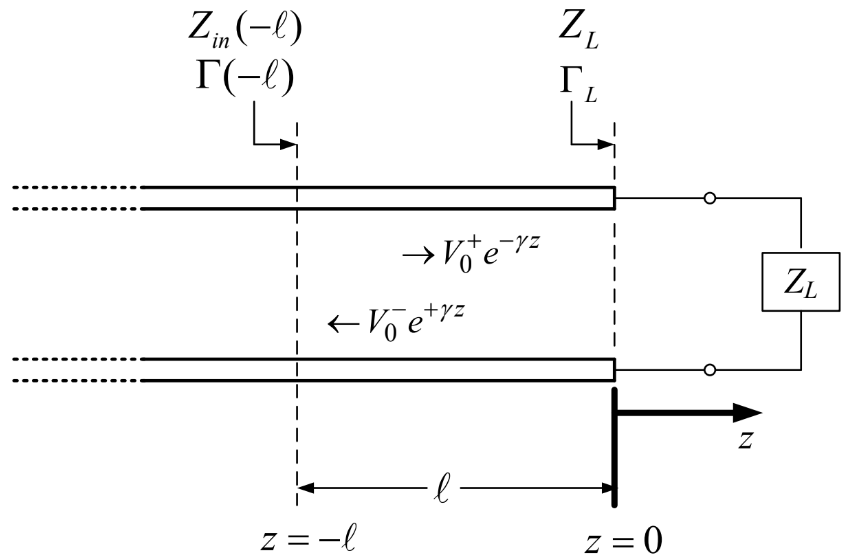
\includegraphics[width=0.7\linewidth]{images/Transmission Line Theory/TL_Load2.png}
    \caption{Transmission line terminated by a load impedance $Z_L$.}
    \label{fig:TL_Load}
\end{figure}

The voltage and current on a transmission line are a superposition of the incident and reflected waves: 
\begin{subequations}
\begin{empheq}[box=\eqnGreenBox]{align}
    \phasor{V}(z) &= V_0^+ e^{-\gamma z} + V_0^- e^{\gamma z} \\ 
    \phasor{I}(z) &= \dfrac{V_0^+}{Z_0} e^{-\gamma z} - \dfrac{V_0^-}{Z_0} e^{\gamma z}
\end{empheq}
\end{subequations}
where $V_0^+$ and $V_0^-$ are complex amplitudes of the incident and reflected waves, respectively. From Fig.\ \ref{fig:TL_Load} we can see that the load impedance is the ratio of the voltage to current at the position $z=0$: 
\begin{equation}
    Z_L = \dfrac{\phasor{V}(0)}{\phasor{I}(0)} = \dfrac{V_0^+ + V_0^-}{V_0^+ - V_0^-} Z_0
\end{equation}
Solving gives 
\begin{empheq}[box=\eqnGreenBox]{equation}
    V_0^- = \dfrac{Z_L - Z_0}{Z_L + Z_0} V_0^+ \label{eq:TLTheory_V0_Reflected}
\end{empheq}
The \coltextit{voltage reflection coefficient} is defined as the ratio of the reflected voltage wave amplitude to the incident voltage wave amplitude. At the load ($z=0$), we denote the reflection coefficient by $\Gamma_L$:
\begin{empheq}[box=\eqnGreenBox]{equation}
    \Gamma_L = \dfrac{V_0^-}{V_0^+} = \dfrac{Z_L - Z_0}{Z_L + Z_0} \label{eq:ReflectionCoefficient}
\end{empheq}
where $\Gamma_L$ is a complex number: $\Gamma_L = |\Gamma_L| e^{j\theta}$. Then, the voltage and current waves on the line may be written as 
\begin{subequations}
\begin{empheq}[box=\eqnGreenBox]{align}
    \phasor{V}(z) &= V_0^+ (e^{-\gamma z} + \Gamma_L e^{\gamma z}) \\ 
    \phasor{I}(z) &= \dfrac{V_0^+}{Z_0} (e^{-\gamma z} - \Gamma_L e^{\gamma z}) 
\end{empheq}
\end{subequations}
It is seen from Eq. (\ref{eq:ReflectionCoefficient}) that the reflection coefficient is zero only if $Z_L = Z_0$. In other words, there is only zero reflection when the load impedance is equal to the characteristic impedance of the line. When $Z_L = Z_0$, we say the load is \textit{matched}. If $Z_L \neq Z_0$, then there is some reflection, and the voltage wave is a superposition of the incident and reflected waves; this is called a \coltextit{standing wave}.  

\begin{note}[Special Load Terminations] When a transmission line is terminated by a matched load, a short circuit, or open circuit, we know what the reflection coefficient will be.
\begin{itemize}
    \item If $Z_L=0$ (short circuit) then $\Gamma_L = -1$ and $|\Gamma_L|=1$.
    \item If $Z_L\to\infty$ (open circuit) then $\Gamma_L$ = 1 and $|\Gamma_L|=1$. 
    \item If $Z_L = Z_0$ (matched load) then $\Gamma_L = 0$. 
    \item If $\Re\{Z_L\} = 0$ (purely reactive load) then $|\Gamma_L|=1$. 
\end{itemize}
\end{note}

An impedance may be normalized to the characteristic impedance. The normalized load impedance $z_L$ is 
\begin{equation}
    z_L = \dfrac{Z_L}{Z_0} = \dfrac{1+\Gamma_L}{1-\Gamma_L}
\end{equation}
A Smith Chart (which is discussed in Section TBD) is an example of where you will see normalized impedances. \par 

At a distance $l$ from the load ($z=-l$), the impedance seen looking towards the load is 
\begin{empheq}[box=\eqnGreenBox]{equation}
    Z_\txtin(-l) = \dfrac{\phasor{V}(-l)}{\phasor{I}(-l)} = Z_0 \left[\dfrac{1+\Gamma_L e^{-2\gamma l}}{1 - \Gamma e^{-2\gamma l}}\right] = Z_0 \left[ \dfrac{Z_L+Z_0\tanh(\gamma l)}{Z_0 + Z_L\tanh(\gamma l)} \right] \label{eq:TLInputImpedance}
\end{empheq}
Similarly, the reflection coefficient at a distance $l$ is 
\begin{empheq}[box=\eqnGreenBox]{equation}
    \Gamma(-l) = \left. \dfrac{V_0^- e^{\gamma z}}{V_0^+ e^{-\gamma z}} \right|_z=-l = \Gamma_L e^{-2\gamma l}
\end{empheq}
The average power on the line can be shown to be 
\begin{empheq}[box=\eqnGreenBox]{equation}
    P_\txtavg = \dfrac{1}{2} \Re\{\phasor{V}(z) \phasor{I}^*(z) \} = \dfrac{1}{2} \dfrac{|V_0^+|^2}{Z_0} (1 - |\Gamma|^2) \label{eq:TLPower}
\end{empheq}
which means that the average power is constant along any point on the line and the total power is equal to the incident minus the reflected. 
\begin{equation}
    P_\txtavg = P_\txtinc - P_\txtrefl
\end{equation}
Note that Eq. (\ref{eq:TLPower}) assumes the generator is matched. \par 

When the load has some mismatch, the load reflects some of the incident power. The loss caused by reflected power is called \coltextit{return loss} (RL). In dB, RL is defined as 
\begin{equation}
    \mathrm{RL}\ [\mathrm{dB}] = -20\log|\Gamma| 
\end{equation}
Recall that we said the waves on the transmission line are standing waves (except when $\Gamma = 0$). So, we define the \coltextit{standing wave ratio} (SWR) which is a ratio of the maximum voltage ampltitude to the minimum amplitude: 
\begin{equation}
    \mathrm{SWR} = \dfrac{V_\txtmax}{V_\txtmin} = \dfrac{1+|\Gamma|}{1-|\Gamma|}
\end{equation}
$\mathrm{SWR}=1$ implies a matched load. 

% --- 
\subsection{Equations for the Lossless Line}
The equations discussed in Section \ref{sec:TerminatedLines} are applicable to lossless transmission lines as well. From Section \ref{sec:LosslessLines}, in a lossless line, $\alpha=0$, which means $\gamma = j\beta$. Therefore, the equations from the previous section remain the same except the following terms are changed: 
\begin{itemize}
    \item $e^{-\gamma l} \longrightarrow e^{-j\beta l}$
    \item $e^{\gamma l} \longrightarrow e^{j\beta l}$
\end{itemize}
For example, we may write the inuput impedance from Eq.\ (\ref{eq:TLInputImpedance}) to be 
\begin{equation}
    Z_\txtin(-l) = \dfrac{\phasor{V}(-l)}{\phasor{I}(-l)} = Z_0 \left[\dfrac{1+\Gamma_L e^{-2j\beta l}}{1 - \Gamma e^{-2j\beta l}}\right] = Z_0 \left[ \dfrac{Z_L+jZ_0\tan(\beta l)}{Z_0 + jZ_L\tan(\beta l)} \right] 
\end{equation}

% *****************************************
% Transmission Line with Load and Source Connected
% *****************************************
\subsection{Transmission Line with Load and Source Connected}

Now a source is connected to a transmission line of length $d$ terminated by a load $Z_L$, as shown in Fig.\ \ref{fig:TLSourceAndLoad}.

\begin{figure}[!htp]
    \centering
    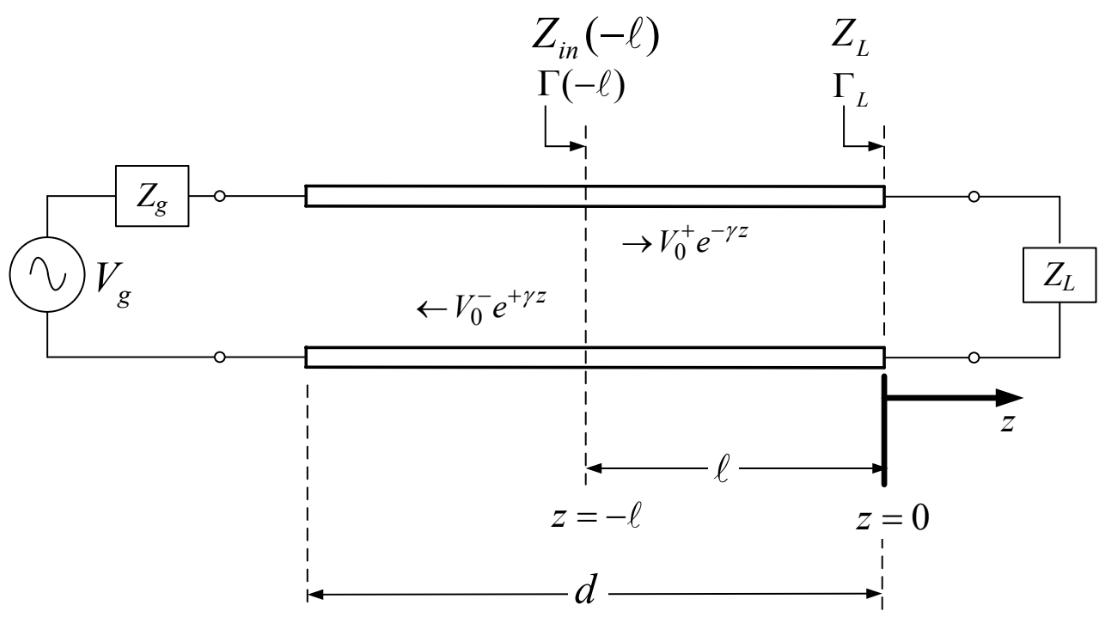
\includegraphics[width=0.8\linewidth]{images/Transmission Line Theory/TL_Source_And_Load.png}
    \caption{Transmission line connected to a source and load.}
    \label{fig:TLSourceAndLoad}
\end{figure}

It can be shown that 
\begin{equation}
    V_0^+ = V_g \left(\dfrac{Z_0}{Z_0+Z_g} \right) \left(\dfrac{e^{-\gamma d}}{1-\Gamma_L\Gamma_G e^{-2\gamma d}} \right)
\end{equation}
where 
\begin{equation}
    \Gamma_G = \dfrac{Z_g - Z_0}{Z_g + Z_0}
\end{equation}
Then, one can find $V_0^-$ by Eqs.\ (\ref{eq:TLTheory_V0_Reflected}), (\ref{eq:ReflectionCoefficient}). The power on the line is 
\begin{equation}
    P_\text{avg}(z) = \dfrac{1}{2} \Re\{\phasor{V}(z) \phasor{I}^*(z) \} = P_i(z) + P_r(z)
\end{equation}
where $P_i(z)$ and $P_r(z)$ denote the incident and reflected power. 
\begin{align}
    P_i(z) &= \dfrac{1}{2} \dfrac{|V_0^+|^2}{Z_0} e^{-2\alpha z} \\ 
    P_r(z) &= \dfrac{1}{2} \dfrac{|V_0^-|^2}{Z_0} e^{2\alpha z}
\end{align}

% *****************************************
% Smith Charts
% *****************************************
\section{Smith Charts}
The Smith chart was invented by P.\ Smith in 1939 and is a graphical tool used to analyze transmission lines. Smith charts are especially useful for impedance matching. \par 

A Smith chart is a polar plot of the complex reflection coefficient with grid lines corresponding to normalized impedances. In Fig.\ \ref{fig:SmithChart2}, we see the basic structure of the Smith chart; the real part of the reflection coefficient ($\Gamma_r$) is along the horizontal axis while the imaginary part ($\Gamma_i$). In Fig.\ \ref{fig:SmithChart_RLXLCircles}, some grid lines corresponding to various impedances are shown on a Smith chart. Fig.\ \ref{fig:SmithChart} shows a typical chart you would use for hand-calculations. \par 

The normalized impedance is represented with a lower-case variable $z$:
\begin{equation}
    z = \dfrac{Z}{Z_0}
\end{equation}
If a lossless transmission line with characteristic impedance $Z_0$ is terminated by a load $Z_L$, the reflection coefficient at the load can be found as 
\begin{equation}
    \Gamma_L = \dfrac{z_L - 1}{z_L + 1} = |\Gamma_L| e^{j\theta}
\end{equation}
where $z_L = Z_L/Z_0$. Or, 
\begin{equation}
    z_L = \dfrac{1+|\Gamma_L|e^{j\theta}}{1-|\Gamma_L|e^{j\theta}}
\end{equation}
The input impedance at a distance $l$ from the load is  
\begin{equation}
    Z_\text{in} = Z_0 \dfrac{1 + \Gamma_L e^{-2j\beta l}}{1 - \Gamma_L e^{-2j\beta l}}
\end{equation}
The normalized input impedance is then 
\begin{equation}
    z_\text{in} = \dfrac{1 + \Gamma_L e^{-2j\beta l}}{1 - \Gamma_L e^{-2j\beta l}}
\end{equation}
A complete rotation around the Smith chart results in a phase change of $2\pi$ in the reflection coefficient, which is equivalent to a

\underline{\textit{Some key points about the Smith chart:
}}
\begin{itemize}
    \item The distance of a point anywhere on the chart to the centre represents the magnitude of the reflection coefficient $\Gamma$. 
    \item The center of the Smith chart ($\Gamma = 0$) corresponds to a matched load (no reflection). Notice how the impedance circle $r_L = 1$ intersects this point. 
    \item The radius of the outermost circle on the chart has a magnitude of 1 ($|\Gamma|=1$). The left and right outermost poitns correspond to the case of short-circuit ($\Gamma=-1$) and open-circuit ($\Gamma=1$). 
    \item In Fig.\ \ref{fig:SmithChart}, you can see 3 scales on the outer perimeter of the circle. The most inner scale represents the phase of the reflection coefficient ($\theta$). The middle scale is the wavelengths towards the load, and the outermost scale is wavelengths towards the generator. 
    \item If you plot a point corresponding to the load impedance, and draw a circle which intersects this point and is centred at the centre of the Smith chart, this is called a SWR circle. The point at which the circle intersects the $\Gamma_r$ axis on the right-hand side is the value of the SWR. Fig.\ \ref{fig:SmithChart_VSWRCircle} illustrates this.
    
\end{itemize}

\underline{\textit{Steps for plotting a reflection coefficient $\Gamma$ on the Smith chart:}}
\begin{enumerate}
    \item Given some $\Gamma_L$ or $Z_L$, first obtain the corresponding normalized impedance $z_L$
    \item Locate the corresponding $r_L$ circle on the Smith chart 
    \item Find the corresponding $x_L$ curve
    \item 
    find where the $r_L$ circle and $x_L$ intersect. Plot your point here. This represents the corresponding reflection coefficient on a Smith chart. 
\end{enumerate}

\begin{figure}[!htp]
    \centering
    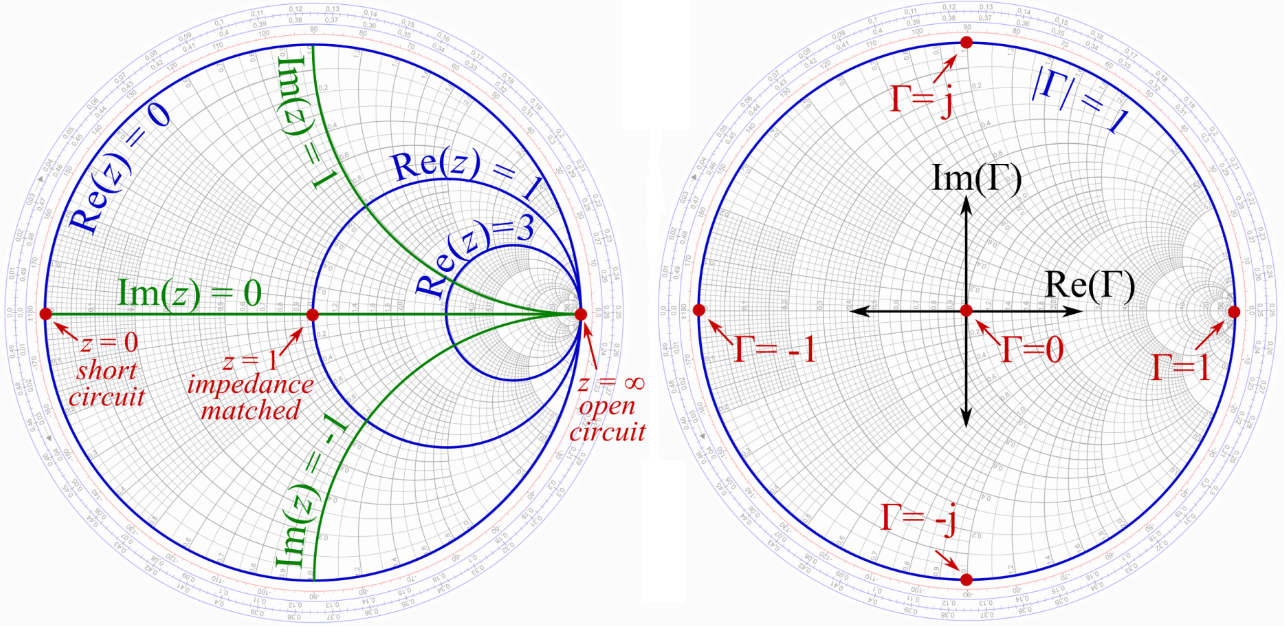
\includegraphics[width=\linewidth]{images/Transmission Line Theory/SmithChart2.png}
    \caption{Smith chart}
    \label{fig:SmithChart2}
\end{figure}

\begin{figure}[!htp]
    \centering
    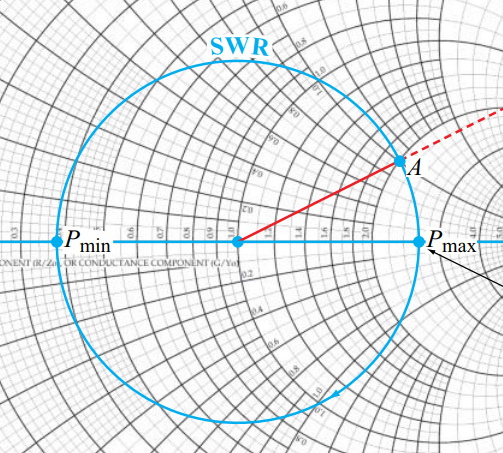
\includegraphics[width=0.5\linewidth]{images/Transmission Line Theory/SmithChart_VSWRCircle.png}
    \caption{VSWR circle on a Smith chart. Point $A$ represents the load impedance. The point $P_\text{max}$ is where the circle intersects the $\Gamma_r$ axis on the right; this is the SWR. In this image, $P_\text{max}$ (and hence SWR) is equal to 2.6.}
    \label{fig:SmithChart_VSWRCircle}
\end{figure}

\begin{figure}[!htp]
    \centering
    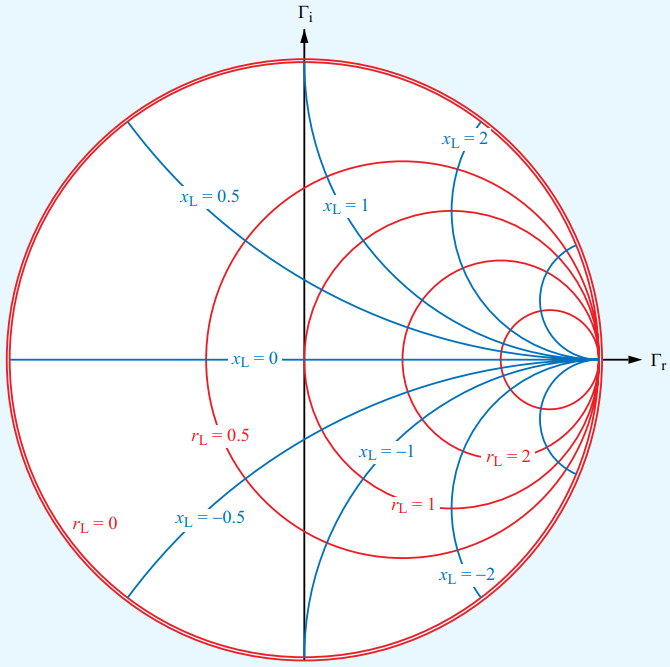
\includegraphics[width=0.5\linewidth]{images/Transmission Line Theory/SmithChart_RLXLCircles.png}
    \caption{Grid lines on a Smith chart corresponding to normalized impedances: $z_L = r_L + j x_L$. }
    \label{fig:SmithChart_RLXLCircles}
\end{figure}

\begin{figure}[!htp]
    \centering
    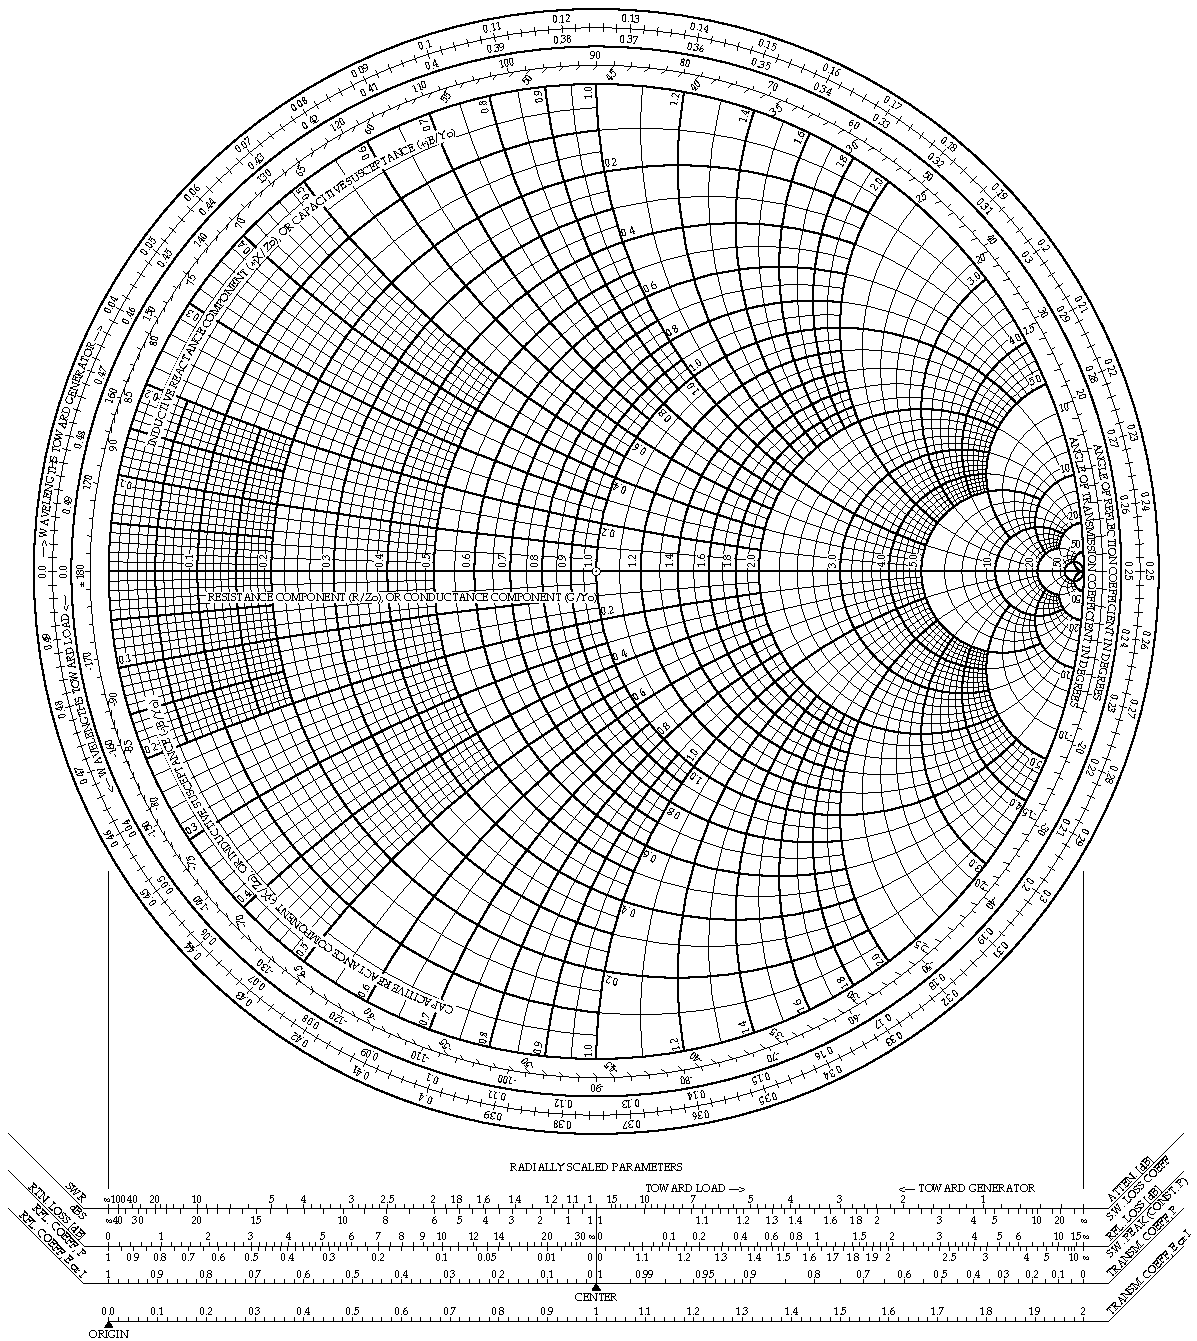
\includegraphics[width=\linewidth]{images/Transmission Line Theory/SmithChart.pdf}
    \caption{The Smith chart}
    \label{fig:SmithChart}
\end{figure}